% !TEX root = ../prospector.tex

\begin{figure}[t]
\centering
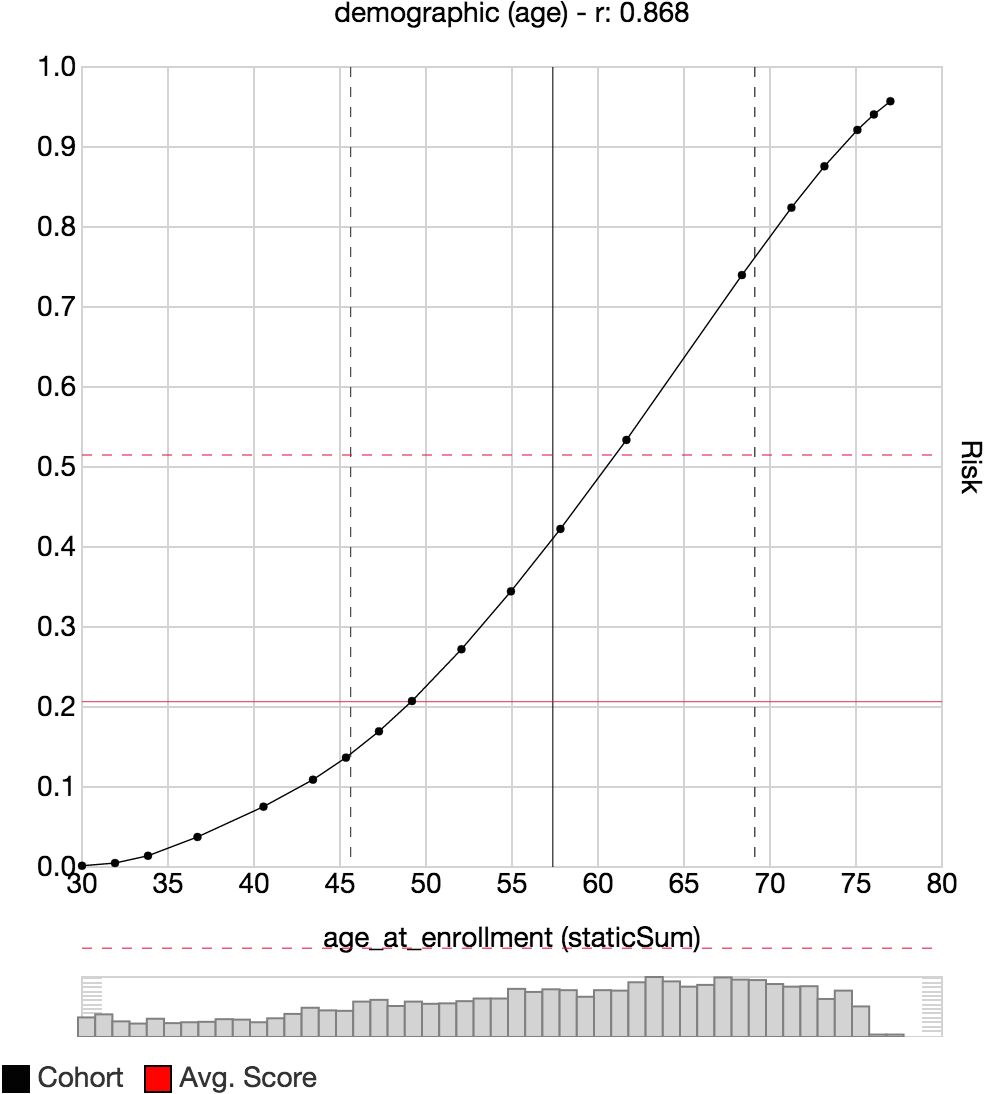
\includegraphics[width=0.55\linewidth]{prospector/pdp_reg} % 0.7
\caption[Partial dependence plots.]{
Partial dependence plots. The black curve shows the average predicted risk
(probability of a certain outcome) if for all rows in the data the value of this
feature was the given value of the horizontal axis.
The red line shows the average predicted risk for the original data.
The vertical line shows the mean of the observed values and the histogram below the plot
shows the distribution of observed values.
Dotted lines show the range of one standard deviation around the mean values.
}
\label{figs:pdp}
\end{figure}

The most widely used technique to understand the relationship between a feature and a prediction is by computing partial dependence \cite{friedman2001,hastie2001}.
The idea of partial dependence plots is to treat predictive models as a black-box and observe how changes in the input affect prediction outcomes.
When inspecting only the partial dependence of one input feature at a time, Formula (\ref{eq:pdp}) can be used to compute a partial dependence plot.

\begin{equation}
pdp_f(v) = \frac{1}{N} \sum_i^N pred(x_i) \;\text{with}\; x_{if} = v
\label{eq:pdp}
\end{equation}

$N$ is the number of rows in the input matrix $x$,
$pred$ is the prediction function that takes one input row, a feature vector, and returns an outcome probability,
and $f$ is the feature used to compute the partial dependence plot.
The formula computes the average outcome over all input rows while changing the value of feature $f$ to the
input value $v$ for each row $x_i$. The original input data is kept fixed. This allows for observing the influence of $f$
on the predicted probabilities.

In order to make this function more concrete, consider the illustrative example in Figure~\ref{figs:pdexplain}, where each input row is a patient, and each column is a feature.  The last column represents the output of the predictive model that predicts if a patient is at low-risk or high-risk for developing Diabetes.  In Figure~\ref{figs:pdexplain}a, the patients' original feature values (age, BMI (Body Mass Index, a standard way to quantify obesity), and glucose level (a standard way to determine Diabetes)) are shown.  If one wants to examine the impact of the glucose feature on the prediction, partial dependence can be applied by keeping all of the other features (age, BMI) as they were, but fixing glucose to a set of fixed values to see how that feature impacts the prediction.  For example, in Figure~\ref{figs:pdexplain}b, the glucose values (highlighted in yellow) are fixed to 100, which yields predictions of only 1 patient being high risk, instead of the original 2.  Conversely, in Figure~\ref{figs:pdexplain}c, glucose is fixed to 180, and 3 patients are predicted to have high risk.  Thus, there appears to be partial dependence of glucose on the prediction.  

Partial dependence is typically visualized as a partial dependence plot, as shown in Figure~\ref{figs:pdp}, which is a line graph that plots the fixed values of the target feature on the x-axis, and the corresponding predicted risk (\ie, probability of a certain outcome) on the y-axis.  
